\documentclass{article}
\usepackage{graphics}
\usepackage{tikz}
\pgfrealjobname{bn}
\begin{document}
% pdflatex --jobname=bn-g bn.tex
\beginpgfgraphicnamed{bn-g}
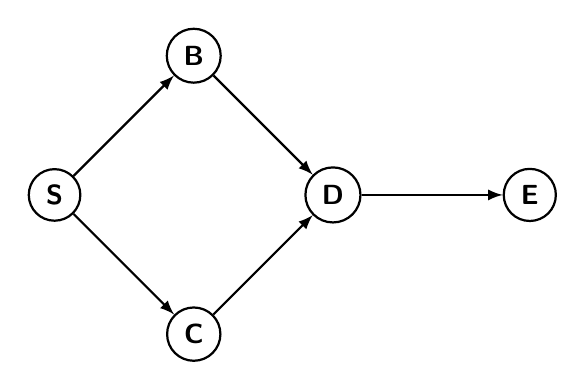
\begin{tikzpicture}[>=latex, node distance=2.5cm, every loop/.style={},
                    thick,main node/.style={circle,draw,font=\sffamily\bfseries}]

  \node[main node] (1) {B};
  \node[main node] (2) [below left of=1] {S};
  \node[main node] (3) [below right of=2] {C};
  \node[main node] (4) [below right of=1] {D};
  \node[main node] (5) [right of=4] {E};

  \path[->][every node/.style={font=\sffamily\small}]
    (1) edge [left] node [left] {} (4)
    (2) edge node [left] {} (1)
        edge node [left] {} (3)
    (3) edge node [] {} (4)
    (4) edge node [right] {} (5);
\end{tikzpicture}
\endpgfgraphicnamed
\end{document}